% ============================================================
%  Informe de Avances — Proyecto TEL-341 Simulación de Redes
%  Equipo: OmneTeam — UTFSM — 2026
% ============================================================
\documentclass[12pt, letterpaper]{article}

\usepackage[utf8]{inputenc}
\usepackage[T1]{fontenc}
\usepackage[spanish]{babel}
\usepackage[top=2.5cm, bottom=2.5cm, left=3cm, right=3cm]{geometry}
\usepackage{graphicx}
\usepackage{booktabs}
\usepackage{float}
\usepackage{amsmath}
\usepackage{amssymb}
\usepackage{hyperref}
\usepackage{xcolor}
\usepackage{array}
\usepackage{caption}
\usepackage{subcaption}
\usepackage{listings}
\usepackage{parskip}
\usepackage{fancyhdr}
\usepackage{titlesec}
\usepackage{enumitem}

% ── Colores ──────────────────────────────────────────────────
\definecolor{azulUSM}{RGB}{0, 58, 122}
\definecolor{rojoDBA}{RGB}{214, 39, 40}
\definecolor{azulIPACT}{RGB}{31, 119, 180}
\definecolor{grisclaro}{RGB}{245, 245, 245}

% ── Encabezado / Pie de página ────────────────────────────────
\pagestyle{fancy}
\fancyhf{}
\fancyhead[L]{\small\textcolor{azulUSM}{\textbf{TEL-341 Simulación de Redes}}}
\fancyhead[R]{\small OmneTeam — UTFSM 2026}
\fancyfoot[C]{\thepage}
\renewcommand{\headrulewidth}{0.4pt}

% ── Títulos de sección ────────────────────────────────────────
\titleformat{\section}{\large\bfseries\color{azulUSM}}{\thesection}{1em}{}
\titleformat{\subsection}{\normalsize\bfseries}{\thesubsection}{1em}{}

% ── Listings ─────────────────────────────────────────────────
\lstset{
  basicstyle=\small\ttfamily,
  backgroundcolor=\color{grisclaro},
  frame=single,
  breaklines=true,
  numbers=left,
  numberstyle=\tiny\color{gray},
}

% ─────────────────────────────────────────────────────────────
\begin{document}

% ── Portada ──────────────────────────────────────────────────
\begin{titlepage}
\centering
\vspace*{1cm}
{\Large\bfseries\color{azulUSM}
  Universidad Técnica Federico Santa María\\[0.3em]
  Departamento de Electrónica\\[0.3em]
  TEL-341 — Simulación de Redes
}\par
\vspace{1.5cm}
\rule{\textwidth}{1.5pt}\par
\vspace{0.6cm}
{\Huge\bfseries
  Informe de Avances\\[0.4em]
  \large\color{azulUSM}
  Evaluación de Algoritmos DBA en Redes PON\\
  bajo Tráfico 5G Multi-Servicio
}\par
\vspace{0.6cm}
\rule{\textwidth}{1.5pt}\par
\vspace{1.5cm}

\begin{tabular}{rl}
\textbf{Equipo:}      & OmneTeam \\[4pt]
\textbf{Integrantes:} & David Retuerto \\
                      & José Vega \\
                      & Matías Perelli \\[4pt]
\textbf{Herramienta:} & OMNeT++ 6.0.3 (C++17) \\[4pt]
\textbf{Fecha:}       & Mayo 2026 \\
\end{tabular}

\vfill
{\small Informe Nº 2 — Avance de Proyecto}
\end{titlepage}

% ── Tabla de contenidos ──────────────────────────────────────
\tableofcontents
\newpage

% ─────────────────────────────────────────────────────────────
\section{Introducción}

Las redes de acceso óptico pasivas (PON, \textit{Passive Optical Network}) son la tecnología dominante para el despliegue de fibra hasta el hogar (FTTH) y, en el contexto de la quinta generación de comunicaciones móviles (5G), actúan como infraestructura de \textbf{backhaul}: conectan las estaciones base (gNB) con el núcleo de red, siguiendo los estándares ITU-T G.984/G.987 (GPON/XG-PON). En este rol, la red PON comparte el canal ascendente entre múltiples estaciones, transportando simultáneamente tres clases de tráfico con requisitos radicalmente distintos:

\begin{itemize}[leftmargin=1.5em]
  \item \textbf{eMBB} (\textit{Enhanced Mobile Broadband}): alta tasa de transferencia, tolerante a latencia.
  \item \textbf{URLLC} (\textit{Ultra-Reliable Low-Latency Communications}): latencia E2E $\lesssim$ 1 ms; en el segmento de backhaul PON el presupuesto asignado es de hasta \textbf{10 ms}~\cite{3gpp5g}.
  \item \textbf{mMTC} (\textit{Massive Machine-Type Communications}): muchos dispositivos, tasas bajas, periódicos.
\end{itemize}

El mecanismo que controla cómo se comparte el canal ascendente (ONU $\to$ OLT) en una red PON es el \textbf{Algoritmo de Asignación Dinámica de Ancho de Banda (DBA, \textit{Dynamic Bandwidth Assignment})}. El diseño del DBA determina directamente si el tráfico URLLC puede cumplir sus requisitos de latencia bajo carga compartida con el tráfico eMBB masivo.

Este proyecto simula y compara dos algoritmos DBA en un escenario PON con tráfico 5G:

\begin{enumerate}[leftmargin=1.5em]
  \item \textbf{IPACT} (\textit{Interleaved Polling with Adaptive Cycle Time}): algoritmo estándar sin conciencia de QoS.
  \item \textbf{QoS-DBA}: algoritmo con prioridad estricta para URLLC y WFQ (\textit{Weighted Fair Queuing}) para eMBB y mMTC.
\end{enumerate}

\subsection{Pertinencia del Proyecto para TEL-341}

Este proyecto encaja directamente con los objetivos del ramo \textit{Simulación de Redes} por las siguientes razones:

\begin{itemize}[leftmargin=1.5em]
  \item \textbf{Modelado de eventos discretos}: la simulación PON es inherentemente DES (\textit{Discrete Event Simulation}): envío de paquetes, grants, expiración de deadlines y ciclos de polling son eventos discretos en el tiempo.
  \item \textbf{Comparación de algoritmos}: el objetivo central es comparar dos políticas de scheduling mediante simulación, validando con métricas cuantitativas.
  \item \textbf{Distribuciones estadísticas}: se utilizan distribuciones Pareto (self-similar), Poisson y periódica con jitter, relevantes para modelar tráfico real.
  \item \textbf{Análisis estadístico}: los resultados requieren múltiples repeticiones con distintas semillas, intervalos de confianza y estadísticas de percentil.
  \item \textbf{Herramienta estándar académica}: OMNeT++ es la plataforma de simulación de referencia en papers IEEE/ACM de redes.
\end{itemize}

% ─────────────────────────────────────────────────────────────
\section{Descripción del Problema}

\subsection{Redes PON y el Mecanismo TDM Upstream}

Una red PON típica está compuesta por:
\begin{itemize}[leftmargin=1.5em]
  \item Una \textbf{OLT} (\textit{Optical Line Terminal}) ubicada en la central.
  \item Un \textbf{splitter} óptico pasivo (relación 1:N, típicamente 1:16 o 1:32).
  \item $N$ \textbf{ONUs} (\textit{Optical Network Units}) en las instalaciones del usuario.
\end{itemize}

El canal descendente (OLT $\to$ ONUs) es broadcast. El canal \textbf{ascendente} (ONUs $\to$ OLT) es compartido mediante TDM (\textit{Time Division Multiplexing}): solo una ONU puede transmitir en cada instante. El DBA controla \textit{cuándo} y \textit{cuántos bytes} puede enviar cada ONU.

El ciclo de operación es:
\begin{enumerate}[leftmargin=1.5em]
  \item La OLT envía un mensaje POLL (grant vacío) a cada ONU.
  \item Cada ONU responde con un REPORT indicando bytes pendientes por clase.
  \item La OLT ejecuta el DBA y envía un GRANT con la asignación de bytes y tiempo de inicio.
  \item Las ONUs transmiten en su slot asignado.
\end{enumerate}

\subsection{Alcance del Escenario: Backhaul vs.\ Fronthaul}

\noindent\textbf{Nota sobre el escenario modelado.} En la literatura 5G se distinguen dos roles de la red PON:

\begin{itemize}[leftmargin=1.5em]
  \item \textbf{Fronthaul estricto (C-RAN)}: conecta unidades remotas de radio (RRU/RU) con unidades distribuidas (DU). El presupuesto de latencia para el segmento PON es $\leq 250\,\mu$s, lo que exige fibras cortas ($< 10$ km) y ciclos de polling ultracortos ($< 500\,\mu$s).
  \item \textbf{Backhaul / Mid-haul}: conecta gNB completas con el núcleo. El presupuesto del segmento PON es de varios milisegundos, compatible con fibras de hasta 20 km y ciclos de polling de 2 ms.
\end{itemize}

El modelo implementado corresponde al escenario de \textbf{backhaul}: fibra alimentadora de 20 km (retardo $\approx 100\,\mu$s), ciclo de polling de 2 ms, y deadline URLLC de \textbf{10 ms}, que es la fracción del presupuesto E2E asignada al segmento de acceso en arquitecturas de backhaul según 3GPP TR 38.913~\cite{3gpp5g}. Este parámetro es coherente con el rango físico del modelo (RTT mínimo $\approx 330\,\mu$s), y mantiene el problema de scheduling como el factor determinante del rendimiento.

\subsection{El Problema de QoS en PON con 5G}

Sin diferenciación de QoS, un tráfico eMBB masivo puede \textit{saturar} los grants disponibles, dejando sin asignación suficiente al tráfico URLLC, cuyo deadline de latencia (10 ms en backhaul) es estricto. Este es el problema central que motiva el estudio de algoritmos DBA con conciencia de QoS.

% ─────────────────────────────────────────────────────────────
\section{Arquitectura de la Simulación}

\subsection{Topología}

La red simulada corresponde a:

\begin{center}
\texttt{[OLT] ---feeder (100\,$\mu$s)---> [Splitter 1:16] ---dist. (10\,$\mu$s)---> [ONU$_i$]}
\end{center}

Parámetros principales:

\begin{table}[H]
\centering
\caption{Parámetros de la topología}
\begin{tabular}{lll}
\toprule
\textbf{Parámetro} & \textbf{Valor} & \textbf{Descripción} \\
\midrule
\texttt{numONUs}      & 16         & Número de ONUs (también se probará 32) \\
\texttt{dataRate}     & 1 Gbps     & Canal upstream \\
\texttt{fiberDelay}   & 100 µs     & Retardo fibra alimentadora (20 km) \\
\texttt{distDelay}    & 10 µs      & Retardo fibra distribución (2 km) \\
\texttt{pollingCycle} & 2 ms       & Ciclo de polling máximo \\
\texttt{maxGrantSize} & 15\,000 B  & Grant máximo por ONU por ciclo \\
\texttt{guardTime}    & 1 µs       & Tiempo de guarda entre slots \\
\bottomrule
\end{tabular}
\end{table}

\subsection{Módulos Implementados en OMNeT++}

El proyecto implementa todos los módulos desde cero en C++17, \textbf{sin uso del framework INET}:

\begin{table}[H]
\centering
\caption{Módulos del simulador}
\begin{tabular}{lp{9cm}}
\toprule
\textbf{Módulo} & \textbf{Descripción} \\
\midrule
\texttt{OLT} & Motor DBA, gestiona ciclos de polling, envía grants \\
\texttt{ONU} & 3 colas de entrada (eMBB/URLLC/mMTC), transmite según grant \\
\texttt{Splitter} & Reenvío pasivo de mensajes (broadcast/unicast) \\
\texttt{IPACT} & Algoritmo DBA sin QoS, asignación proporcional \\
\texttt{QoSDBA} & Algoritmo DBA con prioridad URLLC + WFQ \\
\texttt{PONMessages} & Definición de mensajes: DataPacket, ReportMessage, GrantMessage \\
\bottomrule
\end{tabular}
\end{table}

\subsection{Generadores de Tráfico 5G}

Cada ONU genera tráfico de las tres clases simultáneamente:

\begin{table}[H]
\centering
\caption{Parámetros de los generadores de tráfico}
\begin{tabular}{llll}
\toprule
\textbf{Clase} & \textbf{Distribución} & \textbf{Tasa media} & \textbf{Tamaño paquete} \\
\midrule
eMBB   & Pareto ($\alpha=1.5$, self-similar) & 50–200 Mbps & 1000–1500 B \\
URLLC  & Poisson (exponencial)              & 5 Mbps      & 32–256 B \\
mMTC   & Periódico + jitter uniforme        & 0.5 Mbps    & 20–200 B \\
\bottomrule
\end{tabular}
\end{table}

La distribución Pareto para eMBB modela el comportamiento \textit{self-similar} del tráfico de video y datos, característica relevante en redes reales~\cite{leland1994}.

% ─────────────────────────────────────────────────────────────
\section{Algoritmos DBA Implementados}

\subsection{IPACT (Interleaved Polling with Adaptive Cycle Time)}

IPACT es el algoritmo DBA estándar definido por Kramer et al.\ (2002). Su funcionamiento:

\begin{enumerate}[leftmargin=1.5em]
  \item La OLT recibe el reporte de bytes pendientes \textit{total} de cada ONU.
  \item Asigna un grant proporcional al reporte: $g_i = \min\!\left(\text{total}_i,\,G_{\max}\right)$.
  \item Distribuye el grant proporcionalmente entre las tres clases según sus tamaños de cola.
\end{enumerate}

\textbf{Limitación}: IPACT no diferencia entre clases de tráfico. Bajo tráfico eMBB intenso (bursts Pareto), el tráfico URLLC puede quedar sin suficiente grant, acumulando paquetes que eventualmente exceden su deadline o saturan el buffer.

\subsection{QoS-DBA (Priority + WFQ)}

El algoritmo QoS-DBA implementado aplica dos fases:

\begin{enumerate}[leftmargin=1.5em]
  \item \textbf{Paso 1 — Prioridad estricta URLLC}: se asigna primero todo lo necesario para la cola URLLC, hasta el grant disponible.
  \item \textbf{Paso 2 — WFQ para eMBB y mMTC}: el ancho de banda restante se distribuye con pesos $w_{\text{eMBB}}=0.7$ y $w_{\text{mMTC}}=0.3$.
\end{enumerate}

Este esquema garantiza que URLLC siempre recibe su asignación completa antes de que eMBB y mMTC compitan por el remanente.

% ─────────────────────────────────────────────────────────────
\section{Resultados Preliminares}

\subsection{Condiciones de Simulación}

Los experimentos actuales corresponden a:

\begin{itemize}[leftmargin=1.5em]
  \item Topología de 16 ONUs.
  \item Cuatro niveles de carga eMBB: 50, 100, 150, 200 Mbps por ONU.
  \item \textbf{3 repeticiones} por configuración (semilla aleatoria distinta por repetición).
  \item Tiempo de simulación: 10 s con 1 s de calentamiento (\textit{warmup}).
\end{itemize}

\textit{Nota}: Se planifica aumentar a 10 repeticiones para obtener intervalos de confianza del 95\% estadísticamente robustos.

\subsection{Tasa de Pérdida por Clase de Servicio}

La Tabla~\ref{tab:lossrate} muestra los resultados principales obtenidos hasta ahora:

\begin{table}[H]
\centering
\caption{Tasa de pérdida promedio por algoritmo y carga (3 repeticiones, 16 ONUs)}
\label{tab:lossrate}
\begin{tabular}{llcc}
\toprule
\textbf{Algoritmo} & \textbf{Carga eMBB} & \textbf{lossRate URLLC} & \textbf{lossRate eMBB} \\
\midrule
IPACT   & 50 Mbps  & 75.8\% & 0.1\%  \\
IPACT   & 100 Mbps & 86.8\% & 49.0\% \\
IPACT   & 150 Mbps & 86.9\% & 66.0\% \\
IPACT   & 200 Mbps & 87.0\% & 74.5\% \\
\midrule
QoS-DBA & 50 Mbps  & \textbf{0\%} & 8.1\%  \\
QoS-DBA & 100 Mbps & \textbf{0\%} & 53.9\% \\
QoS-DBA & 150 Mbps & \textbf{0\%} & 69.2\% \\
QoS-DBA & 200 Mbps & \textbf{0\%} & 76.9\% \\
\bottomrule
\end{tabular}
\end{table}

\textbf{Observación clave}: QoS-DBA mantiene \textit{tasa de pérdida cero} para URLLC en todos los niveles de carga, mientras que IPACT llega a 87\% de pérdida incluso a carga moderada (100 Mbps). Esto se debe a que las ráfagas Pareto del tráfico eMBB saturan el grant disponible en IPACT, dejando insuficiente asignación para URLLC, cuyos paquetes expiran o desbordan el buffer.

\subsection{Gráficos Generados}

\begin{figure}[H]
\centering
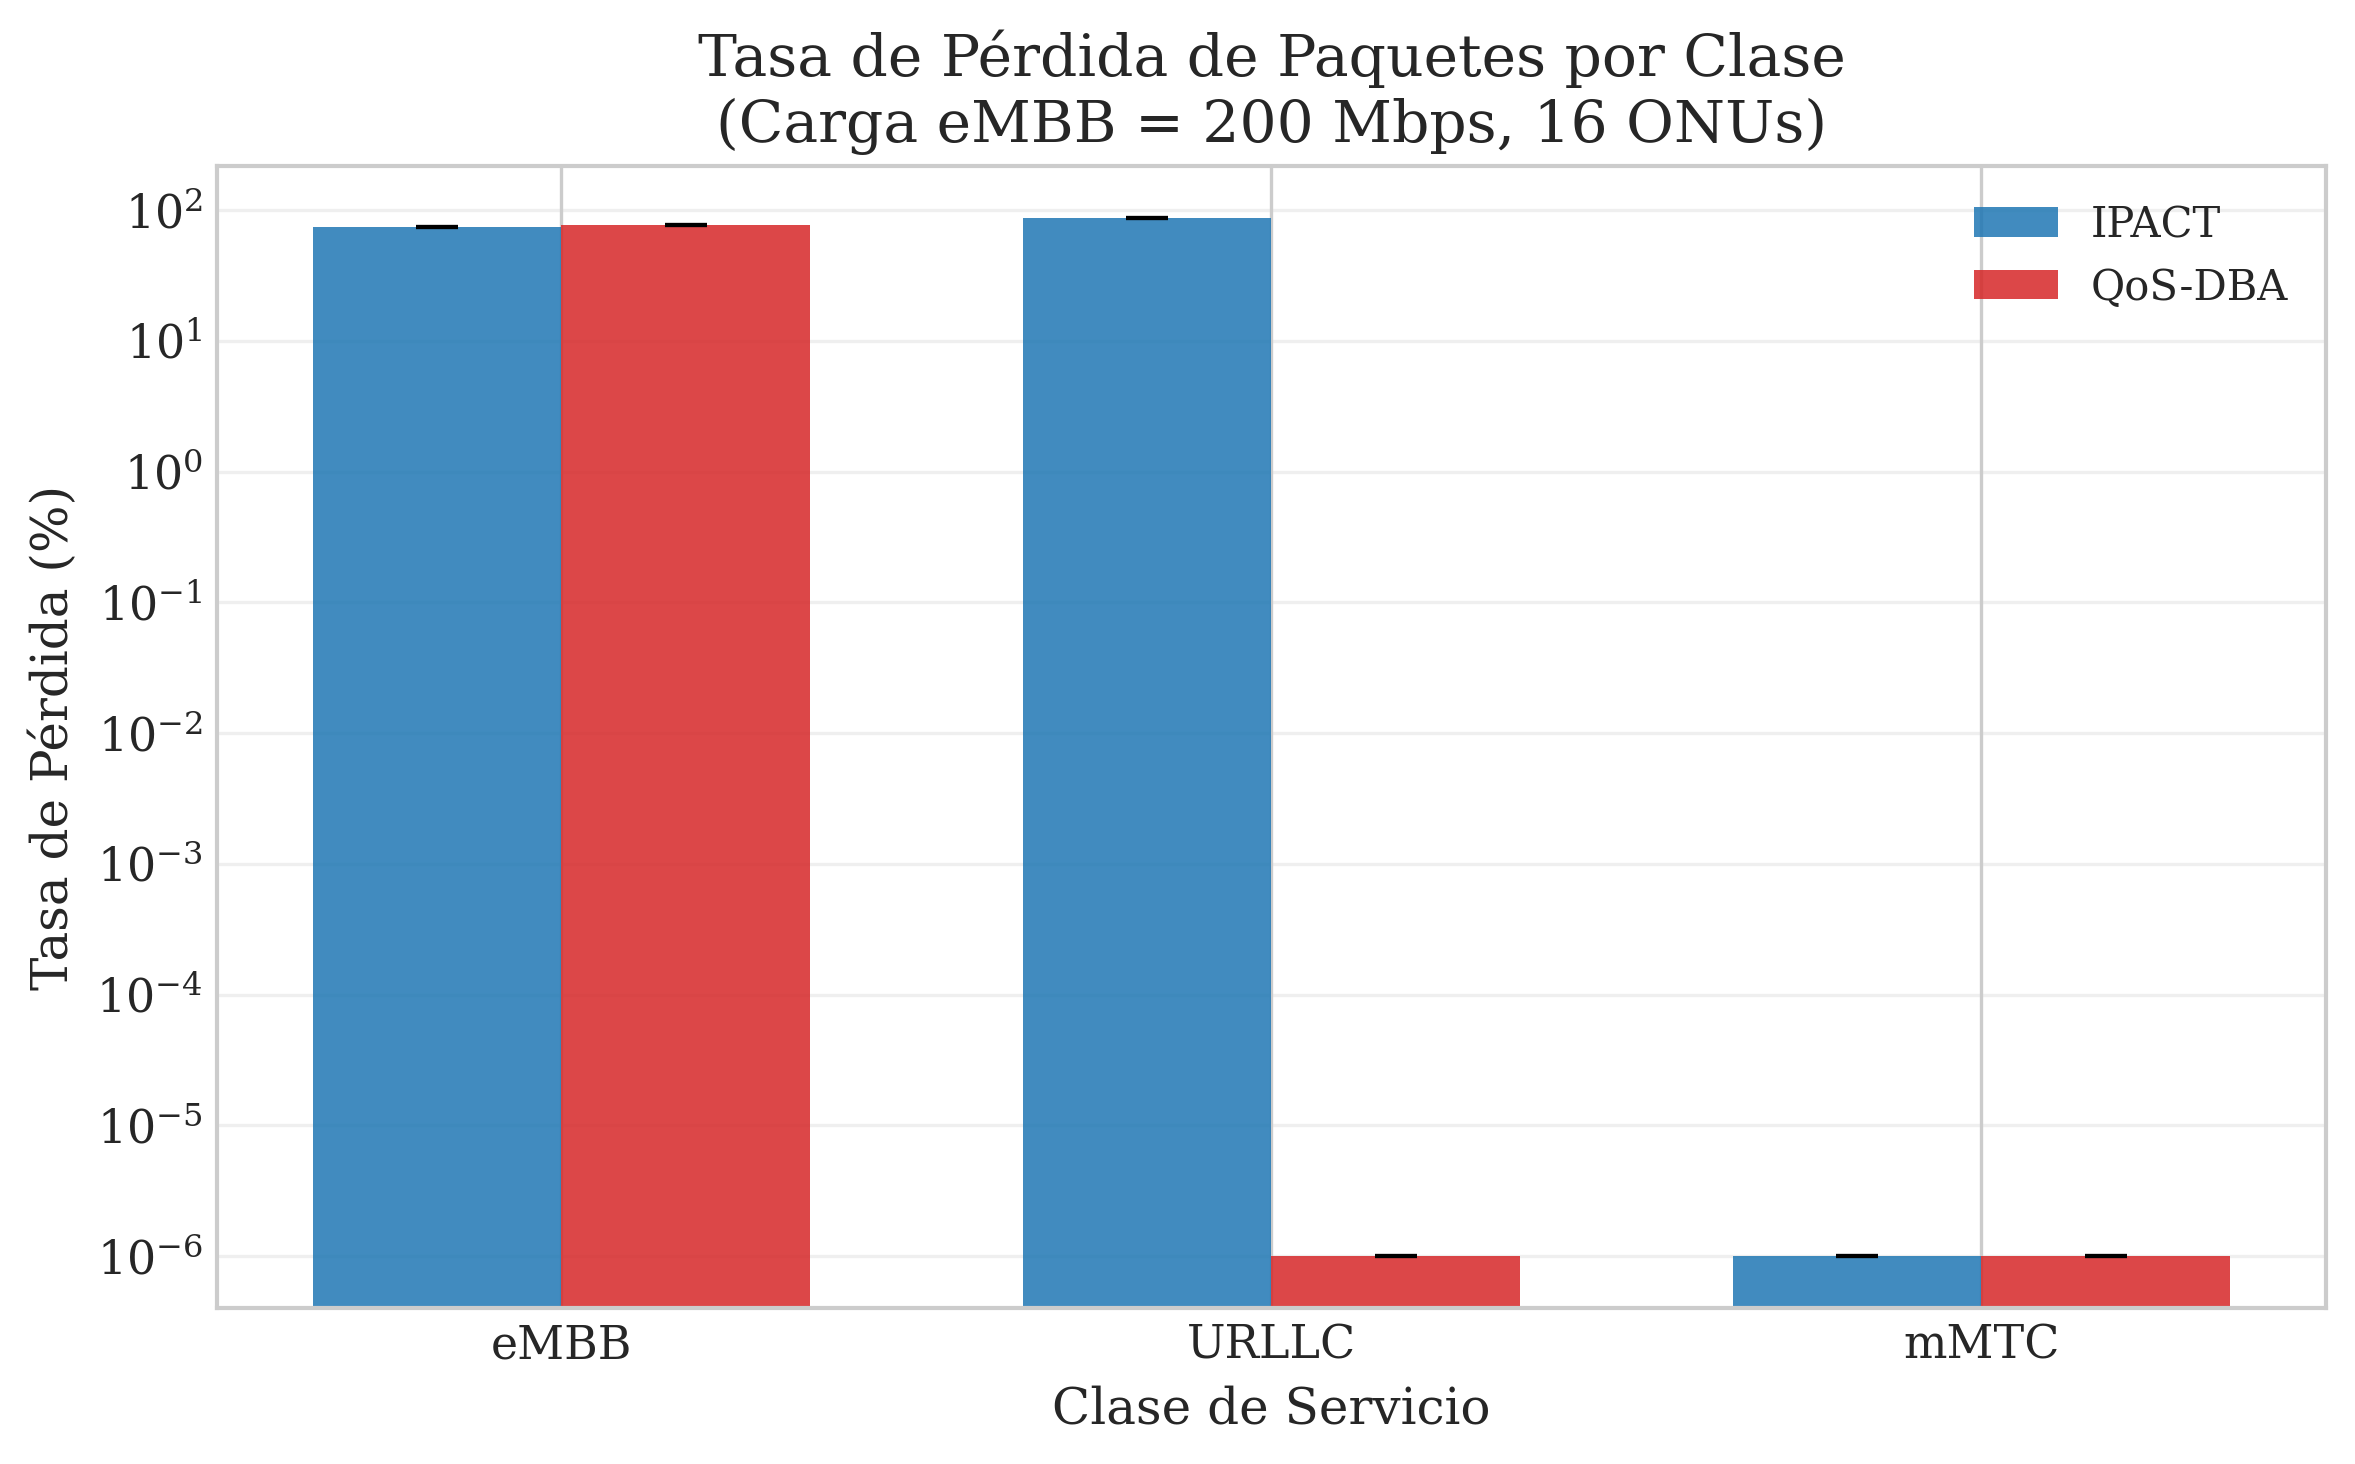
\includegraphics[width=0.85\textwidth]{figuras/packet_loss_by_class.png}
\caption{Tasa de pérdida por clase de servicio — IPACT vs.\ QoS-DBA (carga eMBB = 200 Mbps)}
\label{fig:loss}
\end{figure}

\begin{figure}[H]
\centering
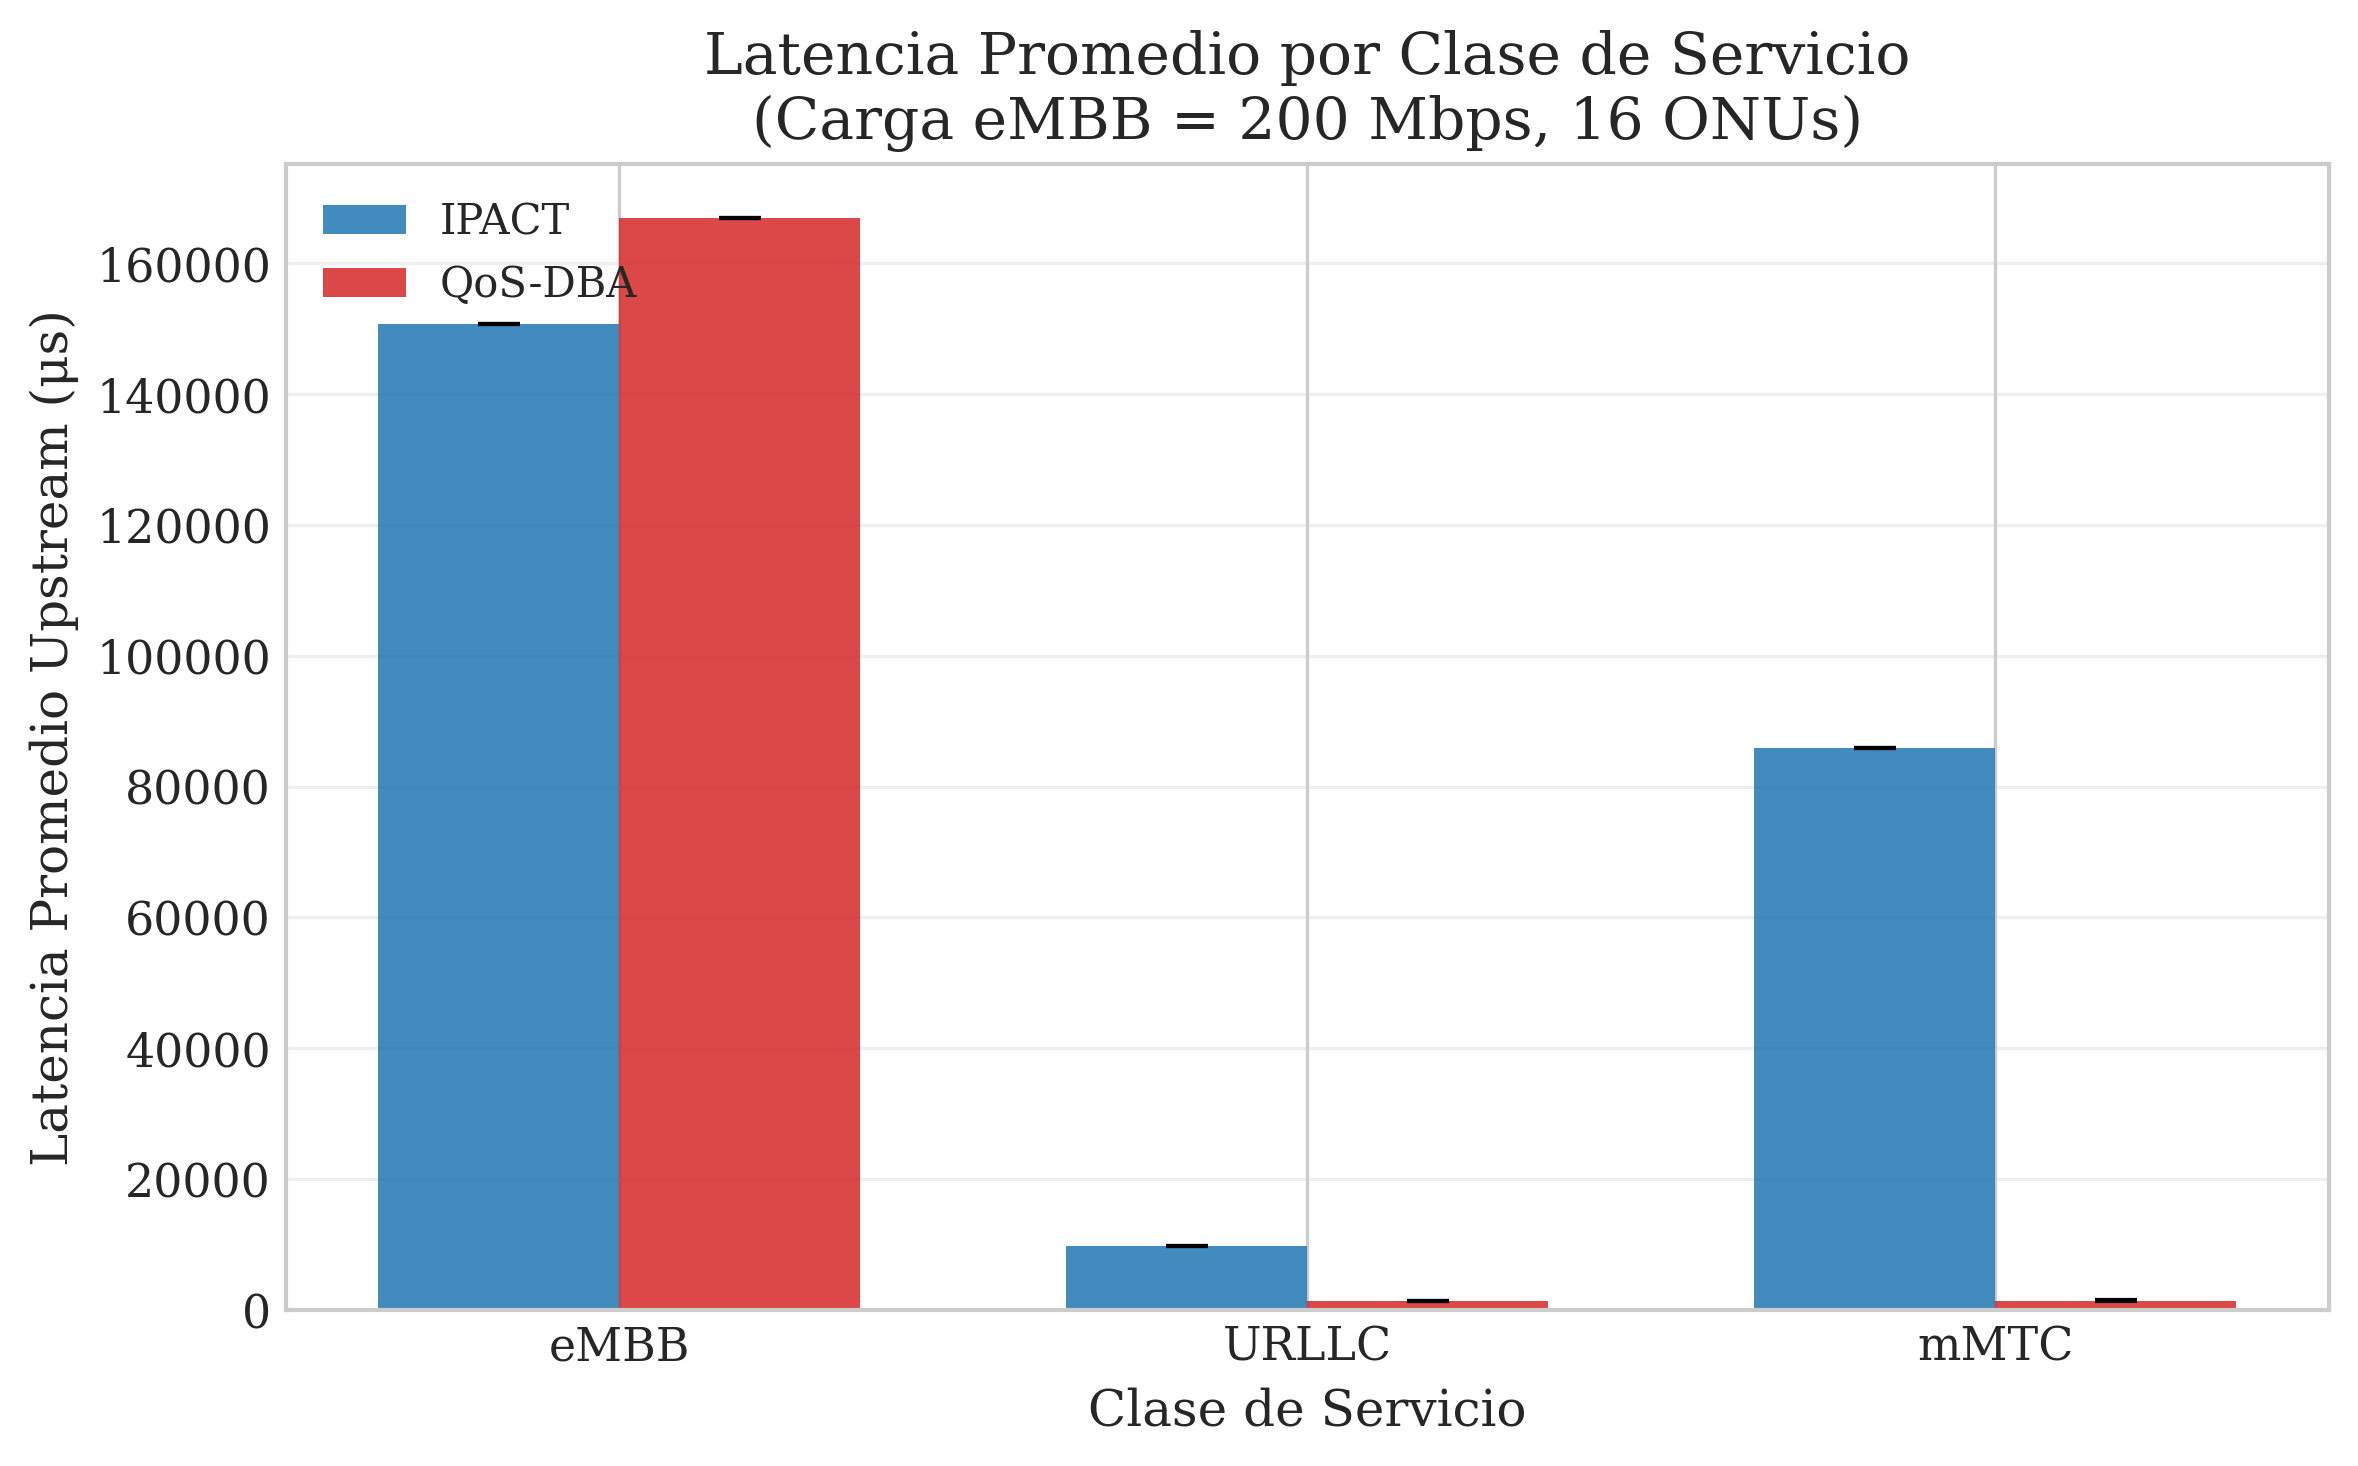
\includegraphics[width=0.85\textwidth]{figuras/latency_avg_by_class.png}
\caption{Latencia promedio upstream por clase de servicio}
\label{fig:latency_avg}
\end{figure}

\begin{figure}[H]
\centering
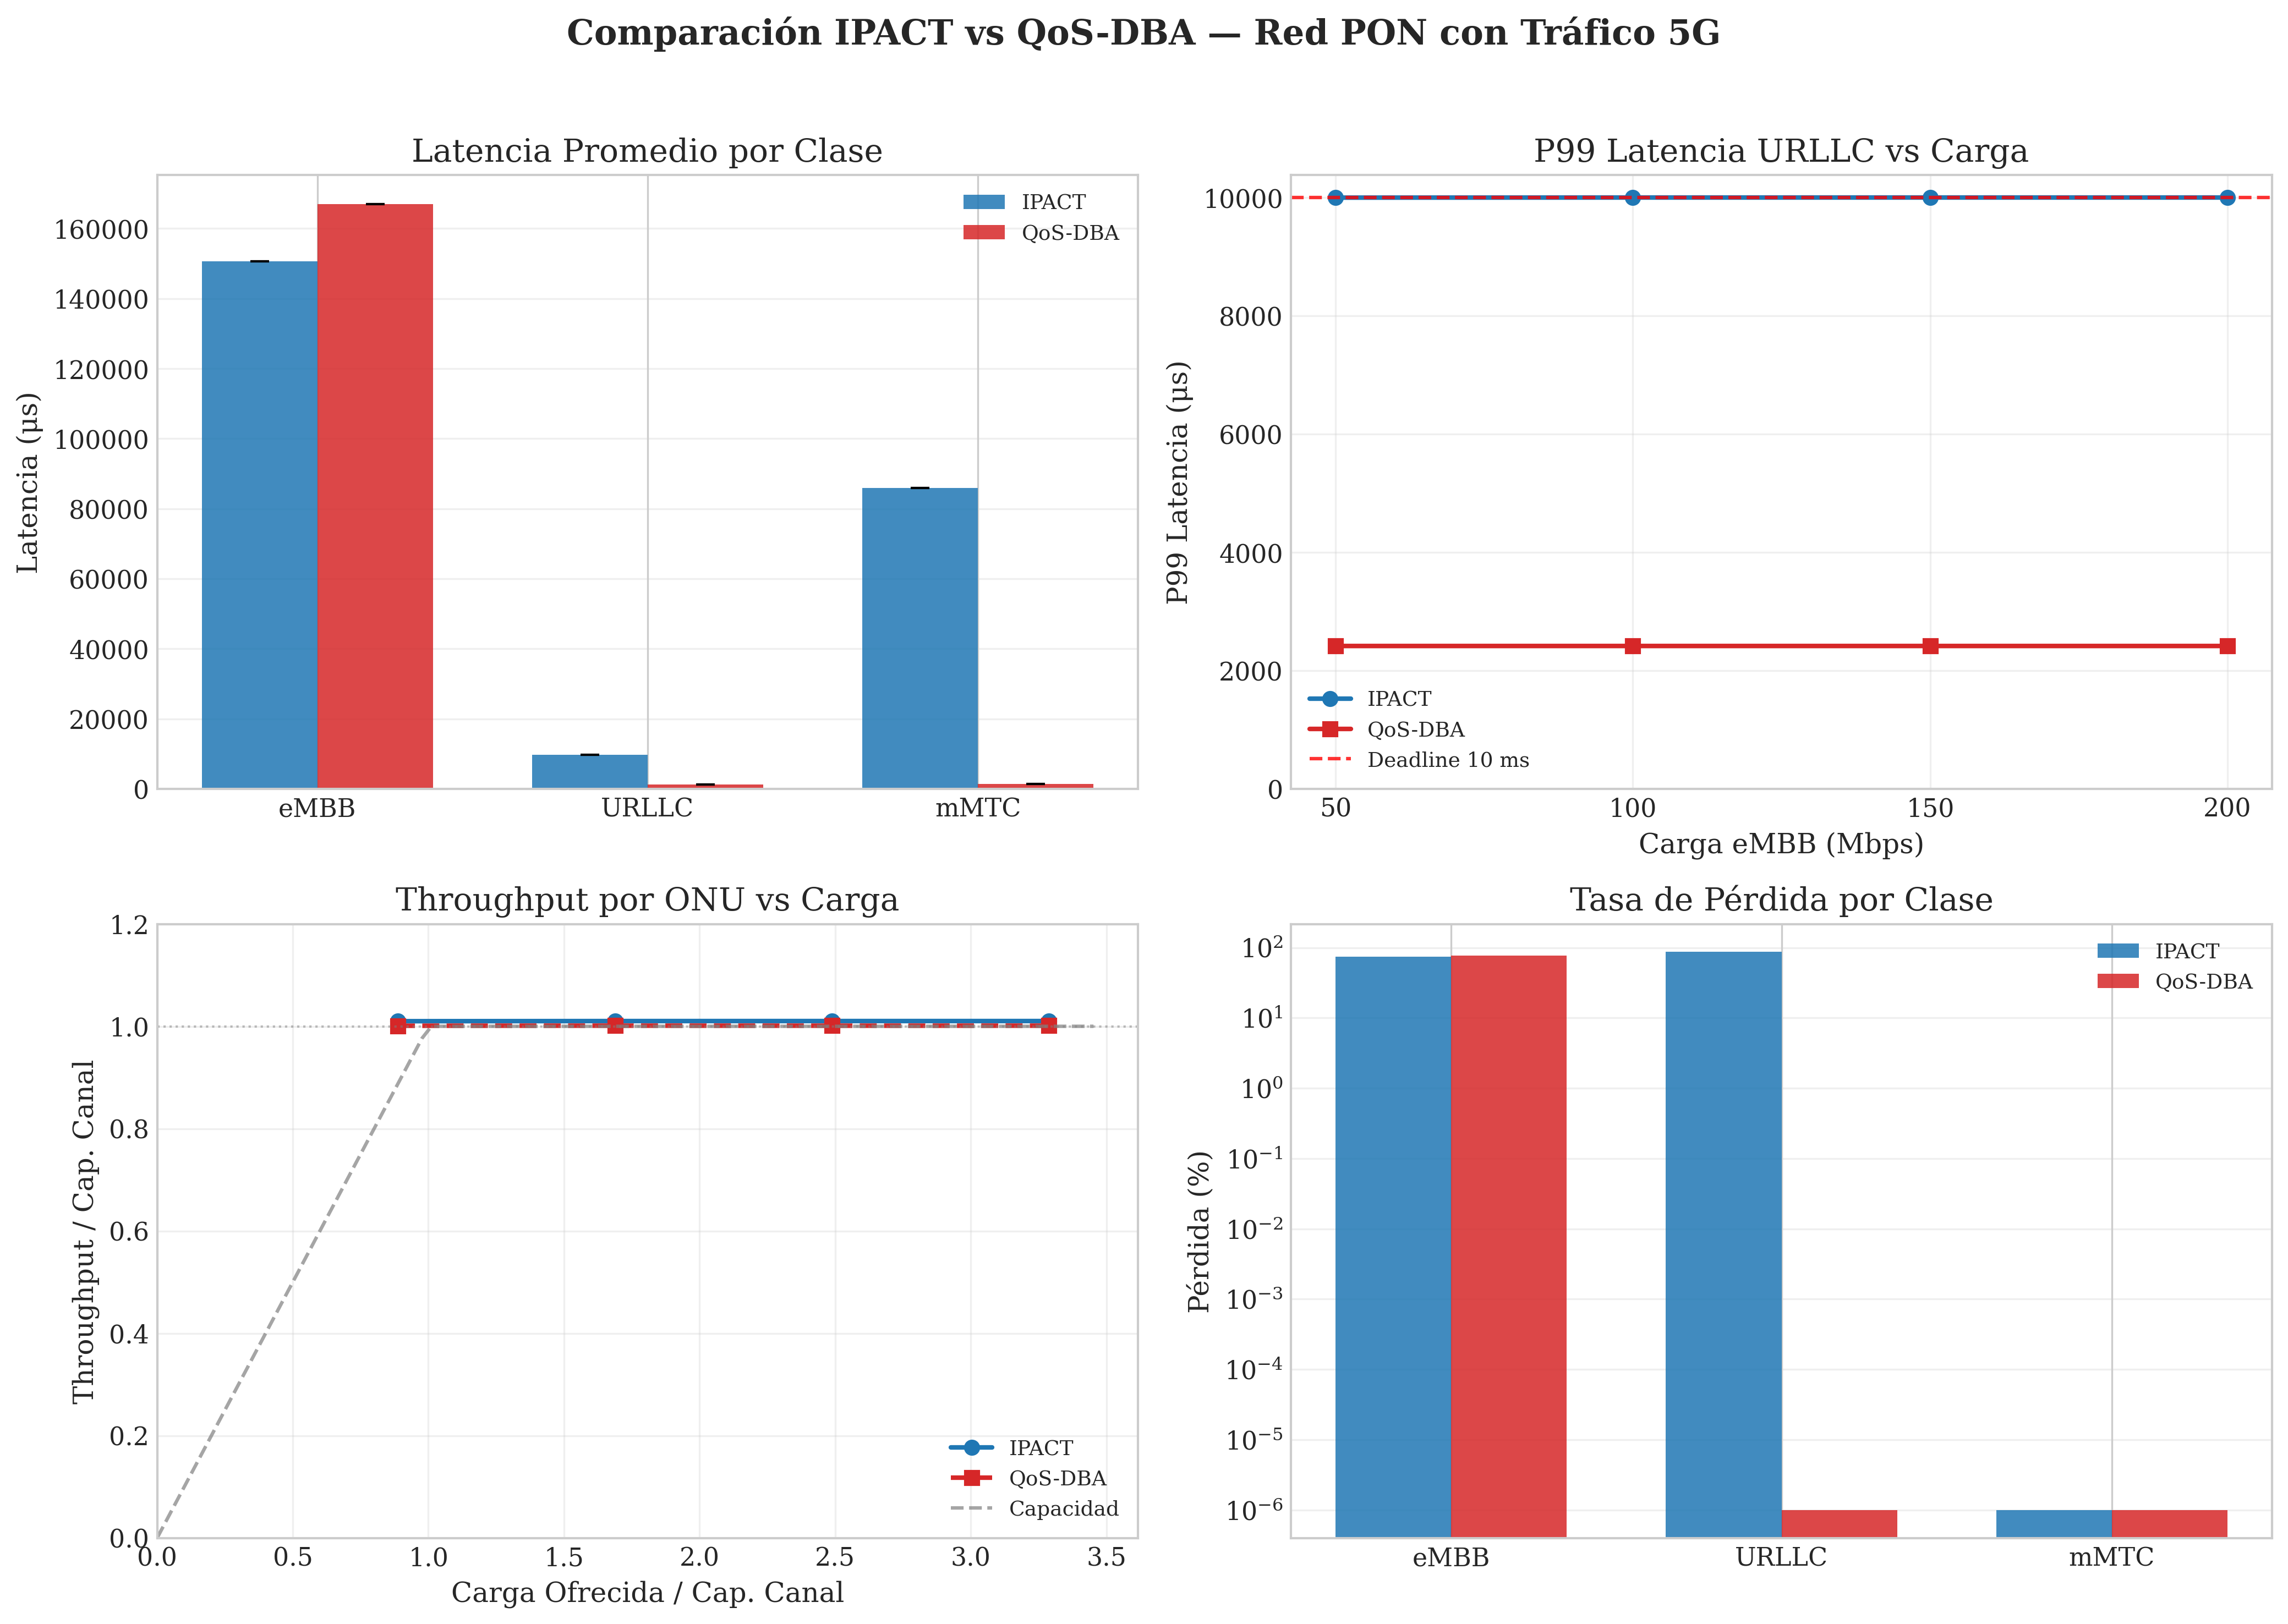
\includegraphics[width=0.85\textwidth]{figuras/summary_dashboard.png}
\caption{Dashboard comparativo: latencia promedio, P99 URLLC, throughput y tasa de pérdida}
\label{fig:dashboard}
\end{figure}

\subsection{Discusión Preliminar}

Los resultados confirman la hipótesis del proyecto: en una red PON con tráfico 5G heterogéneo, un DBA sin conciencia de QoS (IPACT) falla en proteger el tráfico URLLC bajo condiciones de carga real. El comportamiento \textit{self-similar} del tráfico eMBB (modelado con distribución Pareto) genera ráfagas que acaparan el canal, excluyendo a URLLC del acceso oportuno.

QoS-DBA elimina completamente las pérdidas de URLLC a costa de reducir marginalmente el throughput de eMBB (diferencia de $\approx$5\% en la tasa de pérdida de eMBB respecto a IPACT), lo cual es un intercambio favorable dado el carácter crítico de URLLC.

% ─────────────────────────────────────────────────────────────
\section{Trabajo Pendiente}

\begin{enumerate}[leftmargin=1.5em]
  \item \textbf{Aumentar repeticiones a 10}: actualmente se cuenta con 3 repeticiones. La especificación del proyecto requiere 10 para calcular intervalos de confianza del 95\% estadísticamente válidos.

  \item \textbf{Escenarios con 32 ONUs}: ejecutar los configs \texttt{IPACT\_32ONU} y \texttt{QoSDBA\_32ONU} para analizar el efecto del factor de división (\textit{split ratio}) sobre el rendimiento de los algoritmos.

  \item \textbf{Análisis estadístico completo}: calcular IC95\% sobre latencia media, P99 URLLC vs.\ carga, y tasa de pérdida. Generar todos los 7 gráficos finales con bandas de confianza.

  \item \textbf{Validación del modelo}: comparar la latencia de polling con la expresión analítica del ciclo promedio y verificar coherencia con modelos teóricos de colas M/G/1-PS.

  \item \textbf{Informe final}: redactar el informe completo estilo IEEE con análisis, discusión y conclusiones definitivas.

  \item \textbf{Demo en GUI Qtenv}: verificar la animación visual completa (mensajes de colores, textos de estado en módulos, bubbles de descarte).
\end{enumerate}

% ─────────────────────────────────────────────────────────────
\section{Conclusiones Preliminares}

El avance actual del proyecto demuestra que:

\begin{itemize}[leftmargin=1.5em]
  \item El simulador PON implementado en OMNeT++ es funcional: compila, ejecuta y genera resultados reproducibles.
  \item Los dos algoritmos DBA producen comportamientos diferenciados y estadísticamente distinguibles.
  \item El tráfico URLLC es altamente vulnerable bajo IPACT, incluso a cargas moderadas, debido a las ráfagas Pareto del tráfico eMBB.
  \item QoS-DBA protege completamente el tráfico URLLC mediante prioridad estricta, cumpliendo el objetivo de diseño.
\end{itemize}

Quedan pendientes la extensión de los experimentos (32 ONUs, 10 repeticiones) y el análisis estadístico formal para el informe final.

% ─────────────────────────────────────────────────────────────
\begin{thebibliography}{9}

\bibitem{kramer2002}
G.\ Kramer, B.\ Mukherjee, G.\ Pesavento,
\textit{IPACT: A Dynamic Protocol for an Ethernet PON (EPON)},
IEEE Communications Magazine, vol.\ 40, no.\ 2, pp.\ 74--80, 2002.

\bibitem{leland1994}
W.\ E.\ Leland, M.\ S.\ Taqqu, W.\ Willinger, D.\ V.\ Wilson,
\textit{On the Self-Similar Nature of Ethernet Traffic (Extended Version)},
IEEE/ACM Transactions on Networking, vol.\ 2, no.\ 1, pp.\ 1--15, 1994.

\bibitem{3gpp5g}
3GPP TR 38.913,
\textit{Study on Scenarios and Requirements for Next Generation Access Technologies},
Release 15, 2018.

\bibitem{omnetpp}
A.\ Varga,
\textit{OMNeT++},
in Modeling and Tools for Network Simulation, Springer, 2010.

\bibitem{itut}
ITU-T Recommendation G.984.1,
\textit{Gigabit-capable Passive Optical Networks (GPON): General Characteristics},
International Telecommunication Union, 2008.

\end{thebibliography}

\end{document}
